% Nome do capítulo
\chapter{Introdução}
\label{ch:intro}
% Diminuir espaçamento entre título e texto
\vspace{-1.9cm}
% Texto do capítulo

Pesquisas na área de \acf{IHC} tem sido realizadas desde a década de 1960 \cite{myers1998brief}. Hoje interage-se com dispositivos eletrônicos utilizando teclados, \textit{mouses}, acelerômetros e giroscópios, porém, com a popularização de tecnologias de realidade virtual, realidade aumentada e hologramas, foi necessária a criação de novos métodos de \ac{IHC} para que a interação com estes ambientes seja feita de maneira natural e intuitiva para seres humanos. Um dos dispositivos desenvolvidos para esse fim são as luvas eletrônicas que capturam os movimentos dos dedos e posição da mão do usuário através de sensores e os reproduzem em um ambiente tridimensional ou em algum atuador robótico.

A captura dos dados em tempo real é bastante complexa devido à grande variedade de posições que podem ser realizadas e número de variáveis a serem monitoradas, o que requer alto poder computacional. Atualmente exitem alguns dispositivos que atingem esses objetivos, como a \textit{CyberGlove III} que é uma luva eletrônica com até 22 sensores e comunicação sem fio. Outras variedades de luvas eletrônicas como a \textit{Manus VR} ou \textit{Avatar VR} são projetadas para experiências com \acf{RV} e, por isso, utilizam tecnologias baseadas em câmeras ou sensores de infravermelho posicionados no ambiente ao redor do usuário para captar os movimentos. O problema é o alto custo destes dispositivos, variando de US\$250,00 até US\$12.995,00, o que dificulta seu acesso, tanto para fins de pesquisa, quanto para sua utilização prática.

Este trabalho baseia-se no protótipo de uma luva eletrônica de baixo custo desenvolvido por \citeonline{roversi} utilizando a plataforma \textit{Arduino} para aquisição de dados de sensores de flexibilidade e de giroscópios para o controle de uma mão \acf{3D} modelada na plataforma \textit{Unity}. O protótipo desenvolvido possui algumas limitações, não sendo possível detectar movimentos de adução e abdução dos dedos e de desvios radial e ulnar do pulso (Figura \ref{fig:movimentos}), e ainda capta muitos ruídos provenientes do acelerômetro fazendo o modelo virtual da mão oscilar de modo não satisfatório. Este trabalho apresenta um novo protótipo de uma luva eletrônica que capta os movimentos de adução e abdução dos dedos e desvio radial e ulnar do pulso, fazendo uso de duas \textit{Unidades de Medição Inercial} (IMU) e 14 sensores de flexão. Filtros foram aplicados para a suavização das leituras com resultados satisfatórios.

\section{Objetivo Geral}
\label{sec:objg}
O objetivo geral desse trabalho é evoluir o protótipo da luva eletrônica para captura de movimentos de \citeonline{roversi}, com o intuito de incluir os movimentos de adução e abdução dos dedos e desvio radial e ulnar do pulso, reduzir os ruídos captados através de um filtro e melhorar a fixação dos sensores.

\begin{figure}[ht]
% Alterar espaçamentos antes e depois do caption
\setlength{\abovecaptionskip}{0pt}
\setlength{\belowcaptionskip}{0pt}
% Caption
\caption[Movimentos da mão]{Movimentos da mão}
\centering
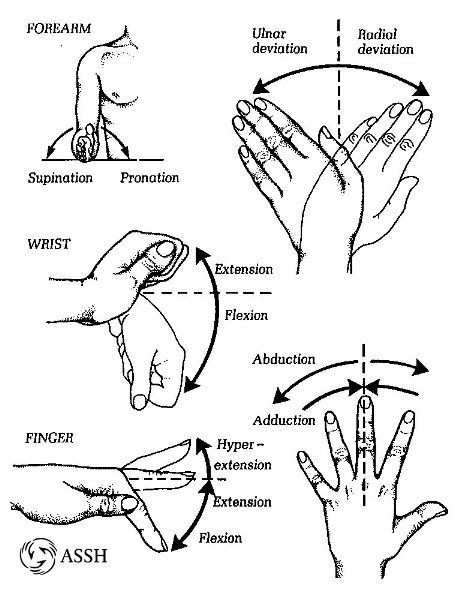
\includegraphics[width=.5\textwidth]{imagem/movimentos}
% Caption centralizada
\captionsetup{justification=centering}
\captionfont{\small{\textbf{\\Fonte: \citeonline{movimentos}}}}	
\label{fig:movimentos}
\end{figure}

\section{Objetivos Específicos}
\label{sec:obje}
Os objetivos específicos deste trabalho consistem em:
  
\begin{compactitem}
	\item[a)] desenvolver um método para captura dos movimentos de adução e abdução dos dedos;
	\item[b)] desenvolver um método para captura dos movimentos de desvios radial e ulnar do pulso;
	\item[c)] aplicar filtros para redução de ruídos dos sensores;
    \item[d)] comparar os resultados com o protótipo de \citeonline{roversi}.
\end{compactitem}

\section{Justificativa}
\label{sec:jus}
Luvas eletrônicas podem ser utilizadas em uma variedade de aplicações. Um caso de uso seria o de médicos que realizam cirurgias e precisam retirar suas luvas para utilizar telas sensíveis ao toque para visualizar informações do paciente. Tais médicos poderiam utilizar luvas eletrônicas para interagir com computadores através de gestos, reduzindo o contato com outros objetos na sala de cirurgia e diminuindo o risco de contaminações. Além disso tais luvas podem ser utilizadas para controle remoto de operadores terminais robóticos, imersão do usuário em um ambiente de \ac{RV} ou reconhecimento de linguagem de sinais. Em cada uma desas aplicações espera-se que os movimentos realizados pelo usuário sejam reproduzidos com fidelidade e precisão, para que a tarefa a ser realizada seja concluída com eficiência.


\section{Organização do Trabalho}
\label{sec:org}
Este trabalho está organizado como segue. O Capítulo \ref{ch:revisao} apresenta tecnologias já existentes e forma a base teórica da pesquisa realizada. A Seção \ref{sec:brac} apresenta um estudo sobre diferentes braços e mãos robóticas. A Seção \ref{sec:luv} apresenta uma comparação entre algumas luvas existentes no mercado. A Seção \ref{sec:sens} mostra os tipos de sensores que podem ser utilizados na construção de luvas eletrônicas. A Seção \ref{sec:trabrel} mostra trabalhos relacionados com o tema proposto. O Capítulo \ref{ch:meto} descreve a solução elaborada para o problema proposto com os requisitos descritos na Seção \ref{sec:requisitos}, os componentes utilizados na Seção \ref{sec:hardware} e os \textit{softwares} utilizados na Seção \ref{sec:software}. O Capítulo \ref{ch:desenvolvimento} apresenta detalhes do desenvolvimento do trabalho, descrevendo o \textit{hardware} na Seção \ref{sec:met_software} e o \textit{software} na Seção \ref{sec:met_software}. No Capítulo \ref{ch:resultados} são apresentadas as análises dos resultados e, por fim, o Capítulo \ref{ch:conclusao} mostra as conclusões e possíveis trabalhos futuros.